\documentclass[11pt,a4paper]{article}

% ---------- Packages ----------
\usepackage[utf8]{inputenc}
\usepackage[T1]{fontenc}
\usepackage{lmodern}
\usepackage{amsmath,amssymb}
\usepackage{enumitem}
\usepackage{geometry}
\usepackage{fancyhdr}
\usepackage[most]{tcolorbox}   % enhanced, breakable
\usepackage{hyperref}

% ---------- Geometry ----------
\geometry{margin=2.5cm}

% ---------- Header/Footer ----------
\setlength{\headheight}{14pt}  % fancyhdr warning verhindern
\pagestyle{fancy}
\fancyhf{}
\lhead{Introduction to Electrical Engineering}
\cfoot{\thepage}

% ---------- Exercise Environment ----------
\newcounter{exercise}
\newenvironment{exercise}[1][]
  {\refstepcounter{exercise}%
   \begin{tcolorbox}[enhanced, breakable, width=\textwidth,
     colback=blue!5!white,colframe=blue!60!black,
     fonttitle=\bfseries\large,
     title=Exercise~\theexercise:~#1]}
  {\end{tcolorbox}}

% ---------- Solution Environment ----------
\newif\ifshowsolutions
\showsolutionstrue  % comment to hide solutions

\newenvironment{solution}
  {\ifshowsolutions
     \begin{tcolorbox}[enhanced, breakable, width=\textwidth,
       colback=green!5!white,colframe=green!50!black,
       fonttitle=\bfseries\large,
       title=Solution]}
  {\end{tcolorbox}\fi}

% ---------- Document ----------
\begin{document}

% ----- Header Box -----
\begin{tcolorbox}[enhanced, breakable, colback=gray!10!white,
  colframe=gray!70!black, fonttitle=\bfseries\large,
  title={Exercise Sheet \#5}, sharp corners, width=\textwidth]
\begin{center}
  Fields 2
\end{center}
\end{tcolorbox}
\vspace{1cm}

% ----- Exercise 1 -----
\begin{exercise}[Time-Dependent Inductor Voltage and Current]
If the voltage waveform below is applied to a $10\text{-mH}$ inductor, find the inductor current $i(t)$ for $0 < t < 2$ seconds. Assume $i(0) = 0$.

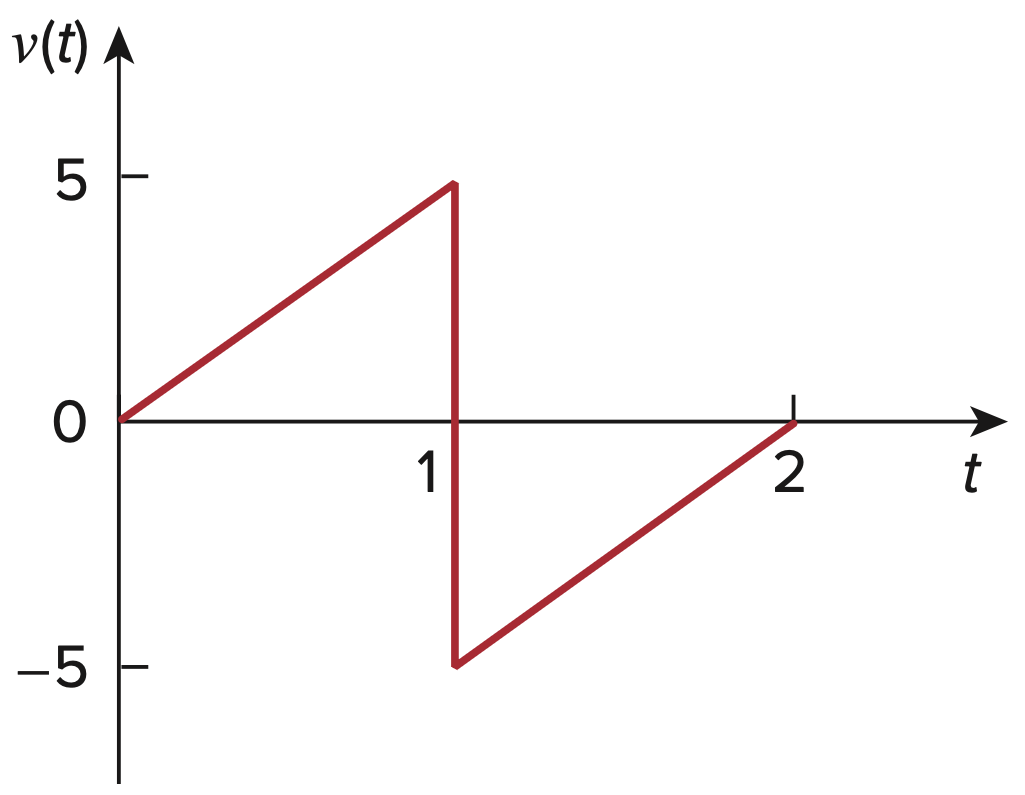
\includegraphics[width=0.5\textwidth]{figures/inductor_VI.png}
\end{exercise}

\ifshowsolutions
\begin{solution}
For an inductor:
\[
v(t) = L \frac{di(t)}{dt}
\]

$0 < t < 1\,\text{s}$ (Ramp up $0$ → $5\,\text{V}$):

\[
v(t) = 5 t\,\mathrm{V} \quad \Rightarrow \quad \frac{di}{dt} = \frac{5 t\,\mathrm{V}}{0.01\,\mathrm{H}} = 500 t\,\mathrm{A/s}
\]

Integrating:
\[
i(t) = \int 500 t\,\mathrm{A/s} \, dt = (250 t^2 + C)\,\mathrm{A}
\]

Since $i(0) = 0$, $C=0$:
\[
\boxed{i(t) = 250 t^2\,\mathrm{A}, \quad 0 < t < 1}
\]

\bigskip

$t = 1\,\text{s}$ (instantaneous drop $5$ → $-5\,\text{V}$):

An ideal inductor cannot change current instantaneously. Therefore, the inductor current is continuous at $t=1$:
\[
i(1^-) = i(1^+) = 250\,\text{A}
\]

The instantaneous voltage jump produces a finite slope change in $di/dt$, $i(t)$ itself is continuous.

\bigskip

$1 < t < 2\,\text{s}$ (ramp from $-5$ → $0\,\text{V}$):

Voltage is now
\[
v(t) = -5\,\text{V} + 5 (t-1)\,\text{V} = (5 t - 10)\,\text{V}, \quad 1 < t < 2.
\]

Then
\[
\frac{di}{dt} = \frac{(5 t - 10)\,\text{V}}{0.01,\mathrm{H}} = (500 t - 1000)\,\mathrm{A/s}.
\]

Integrate:
\[
i(t) = \int (500 t - 1000)\,\mathrm{A/s} dt = (250 t^2 - 1000 t + C)\,\mathrm{A}
\]

Use continuity at $t = 1$: $i(1) = 250\,\mathrm{A}$
\[
250\,\mathrm{A} = (250(1)^2 - 1000(1) + C)\,\mathrm{A} \implies C = 1000
\]

So:
\[
\boxed{i(t) = (250 t^2 - 1000 t + 1000)\,\mathrm{A}, \quad 1 < t < 2}
\]
\end{solution}
\fi

% ----- Exercise 2 -----
\begin{exercise}[Coil]
A cylindrical coil with a length of $2.7 \,\mathrm{m}$, a radius of $0.85 \,\mathrm{cm}$, and 600 turns carries a current of $2.5 \,\mathrm{A}$. Calculate $B$ inside the coil, far from its ends.
\end{exercise}

\ifshowsolutions
\begin{solution}
The magnetic field inside a long solenoid (far from its ends) is given by
\[
B = \mu_0 \, n \, I,
\]
where $n$ is the number of turns per unit length:
\[
n = \frac{N}{l} = \frac{600}{2.7 \,\mathrm{m}} \approx 222.22 \,\mathrm{turns/m}
\]

With the permeability of free space
\[
\mu_0 = 4\pi \cdot 10^{-7} \,\mathrm{H/m},
\]
the magnetic field is:
\[
B = (4 \pi \cdot 10^{-7}) \cdot 222.22 \cdot 2.5 \,\mathrm{T} = 6.98 \cdot 10^{-4} \,\mathrm{T} \approx 0.7 \,\mathrm{mT}
\]
\end{solution}
\fi

% ----- Exercise 3 -----
\begin{exercise}[Energy of Inductors]
The current in an 80-mH inductor increases from 0 to 60 mA (steady state). How much energy is stored in the inductor?
\end{exercise}

\ifshowsolutions
\begin{solution}
The energy stored in the inductor is given by
\[
W = \frac{1}{2} L I^2 = \frac{1}{2} (0.08) (0.06)^2~\text{J} = 144~\mu\text{J}.
\]
\end{solution}
\fi

% ----- Exercise 4 -----
\begin{exercise}[Inductor and Capacitor under DC]
For the circuit below, calculate the value of $R$ that will make the energy stored in the capacitor the same as that stored in the inductor under DC condtitions.

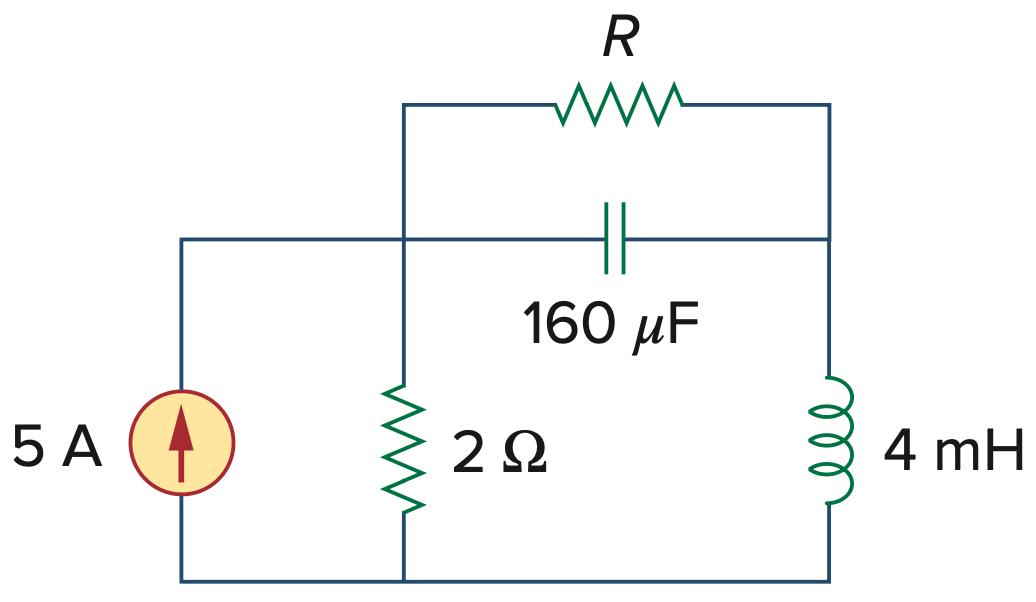
\includegraphics[width=0.7\textwidth]{figures/inductor_capacitor_circuit.png}
\end{exercise}

\ifshowsolutions
\begin{solution}
Under steady-state DC, the capacitor is an open circuit and the inductor is a short circuit. Call the top node voltage \(V\). The \(2\text{-}\Omega\) resistor and \(R\) both go to ground, so
\[
\frac{V}{R} + \frac{V}{2\,\Omega} = 5\,\mathrm{A} \quad \Rightarrow \quad V = \frac{10R}{R+2}.
\]

The inductor DC current is the current through \(R\):
\[
I_L = \frac{V}{R} = \frac{10}{R + 2}
\]

Equate stored energies:
\[
\frac{1}{2} C V^2 = \frac{1}{2} L I_L^2
\]

Substituting \(V\) and \(I_L\) gives
\[
C \left( \frac{10 R}{R + 2} \right)^2 = L \left( \frac{10}{R + 2} \right)^2 \quad \Rightarrow \quad C R^2 = L,
\]

and therefore

\[
R = \sqrt{\frac{L}{C}} = \sqrt{\frac{4 \times 10^{-3}}{160 \times 10^{-6}}}\,\Omega = 5\,\Omega.
\]
\end{solution}
\fi

% ----- Exercise 5 -----
\begin{exercise}[Series and Parallel Inductors]
Determine $L_{\text{eq}}$ at terminals a-b of the circuit below.

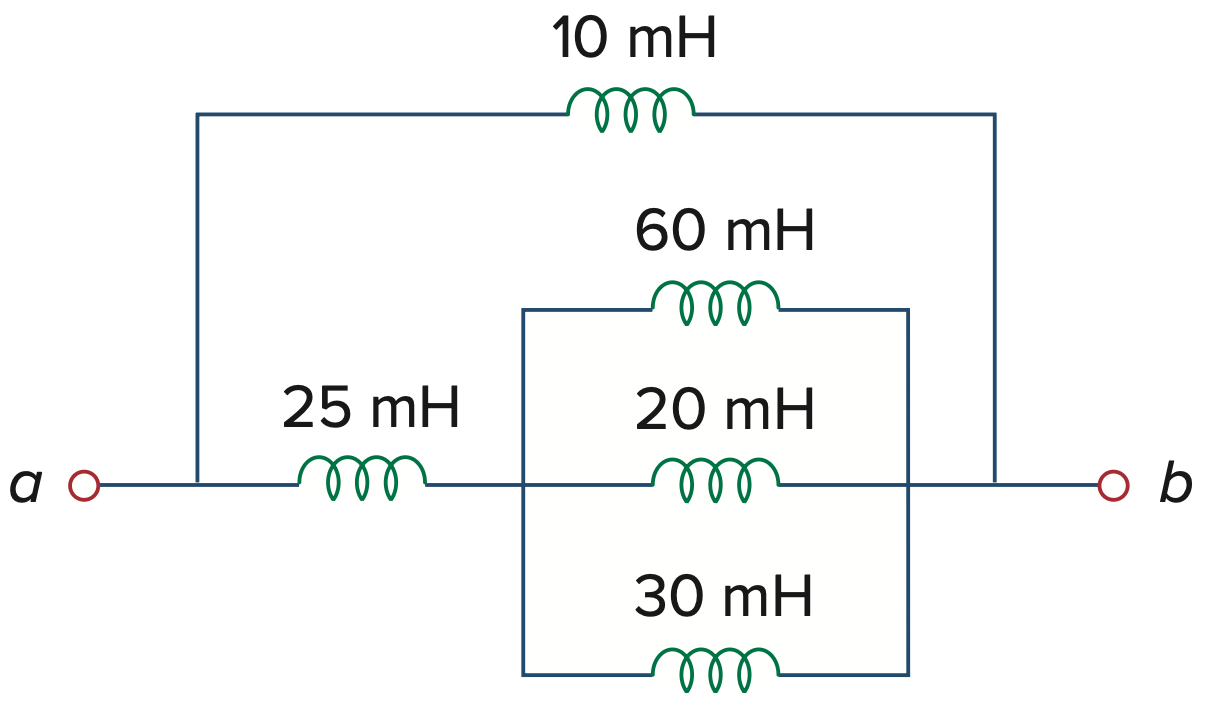
\includegraphics[width=0.7\textwidth]{figures/inductors_circuit.png}
\end{exercise}

\ifshowsolutions
\begin{solution}
Step 1: Parallel combination of the three inductances with $60~\text{mH}$, $20~\text{mH}$, $30~\text{mH}$:
\[
\frac{1}{L_{\text{p}}} = \frac{1}{60~\text{mH}} + \frac{1}{20~\text{mH}} + \frac{1}{30~\text{mH}} = \frac{1}{10}~\frac{1}{\text{mH}}
\]
\[
\Rightarrow L_{\text{p}} = 10~\text{mH}
\]

Step 2: Series combination with the inductance of $25~\text{mH}$:
\[
L_{\text{s}} = L_{\text{p}} + 25~\text{mH} = 10~\text{mH} + 25~\text{mH} = 35~\text{mH}
\]

Step 3: Parallel combination with the inductance of $10~\text{mH}$:
\[
\frac{1}{L_{\text{eq}}} = \frac{1}{L_{\text{s}}} + \frac{1}{10~\text{mH}} = \frac{1}{35~\text{mH}} + \frac{1}{10~\text{mH}} = \frac{9}{70}~\frac{1}{\text{mH}}
\]
\[
\Rightarrow L_{\text{eq}} \approx 7.78~\text{mH}
\]
\end{solution}
\fi

% ----- Exercise 6 -----
\begin{exercise}[Ideal Transformer]
A 480-V to 2400-V step-up ideal transformer delivers $50\,\text{kW}$ to a resistive load. Calculate:
\begin{enumerate}[label=\alph*)]
  \item the turns ratio
  \item the primary current
  \item the secondary current
\end{enumerate}
\end{exercise}

\ifshowsolutions
\begin{solution}
\begin{enumerate}[label=\alph*)]
\item Turns ratio (primary to secondary):
\[
\alpha = \frac{V_P}{V_S} = \frac{480\,\text{V}}{2400\,\text{V}} = 0.2
\]
\item Primary current:
\[
I_P = \frac{P}{V_P} = \frac{50000\,\text{W}}{480\,\text{V}} \approx 104.17\,\text{A}
\]
\item Secondary current:
\[
I_S = \frac{P}{V_S} = \frac{50000\,\text{W}}{2400\,\text{V}} \approx 20.83\,\text{A}
\]
Check:
\[
\frac{I_S}{I_P} \approx 0.2
\]
\end{enumerate}

\textbf{Remark:}
For AC, one would simply consider RMS values.
\end{solution}
\fi

% ----- Exercise 7 -----
\begin{exercise}[Mutual Inductance]
For the three coupled coils below, calculate the total inductance.

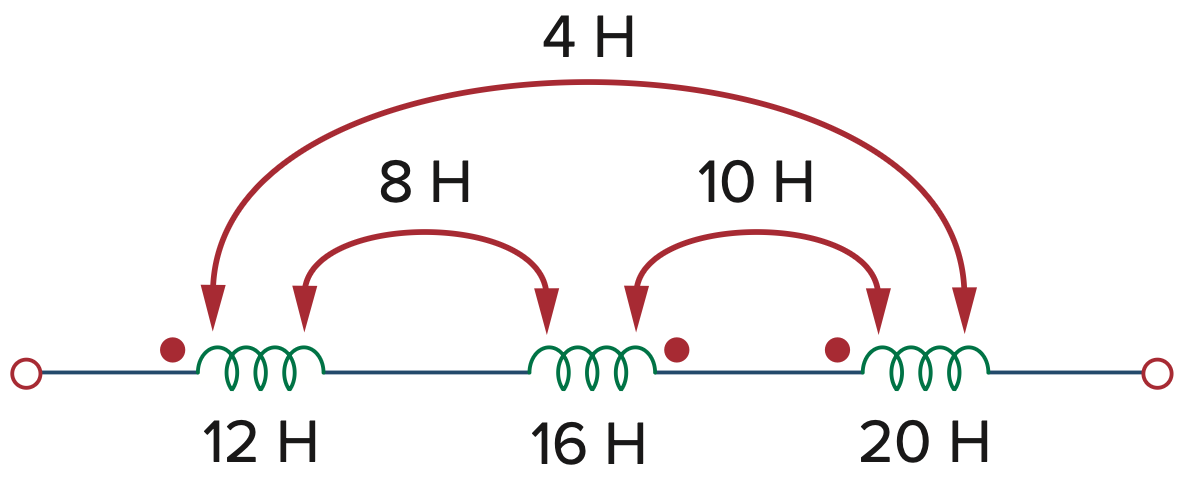
\includegraphics[width=0.7\textwidth]{figures/mutual_inductance.png}

\textbf{Background:}
The polarity of the mutual voltage is defined by the orientation or particular way in which the two coils are physically wound. It can be determined by applying Lenz’s law in conjunction with the right-hand rule. In circuit diagrams, the polarity is often shown by the dot convention: A dot is placed in the circuit at one end of each of the two magnetically coupled coils to indicate the direction of the magnetic flux if current enters that dotted terminal of the coil. The convention then reads: If a current enters the dotted terminal of one coil, the reference polarity of the mutual voltage in the second coil is positive at the dotted terminal of the second coil.
\end{exercise}

\ifshowsolutions
\begin{solution}
\[
\text{Given: } 
\begin{cases}
L_1 = 12~\text{H},\\
L_2 = 16~\text{H},\\
L_3 = 20~\text{H},\\
M_{12} = 8~\text{H},\\
M_{23} = 10~\text{H},\\
M_{13} = 4~\text{H}.
\end{cases}
\]

The total inductance of a system of magnetically coupled coils connected in series depends not only on the self-inductances of the coils, but also on the mutual inductances between them.  

When two coils are connected such that the magnetic flux produced by one \emph{aids} the flux in the other, the mutual inductance contributes \emph{positively}. If the fluxes \emph{oppose} each other, the mutual inductance contributes \emph{negatively}.

In the given circuit:
\begin{enumerate}
  \item The dots indicate the polarity of the induced voltage in each coil.
  \item The connection pattern shows that:
  \begin{enumerate}
    \item \( M_{12} \) and \( M_{23} \) are \emph{opposing} (the current enters the dotted terminal of one coil and leaves the dotted terminal of the other).
    \item \( M_{13} \) is \emph{aiding} (the current enters both dotted terminals).
  \end{enumerate}
\end{enumerate}

For three series-connected coupled coils, the equivalent inductance is given by:
\[
L_{\text{eq}} = L_1 + L_2 + L_3 + 2(\pm M_{12} \pm M_{23} \pm M_{13}),
\]
where the signs depend on whether the mutual coupling is aiding or opposing.

From the polarity information in the diagram, we have:
\[
L_{\text{eq}} = L_1 + L_2 + L_3 + 2(M_{13} - M_{12} - M_{23}) = (12 + 16 + 20 + 2(4 - 8 - 10))~\text{H} = 20~\text{H}
\]

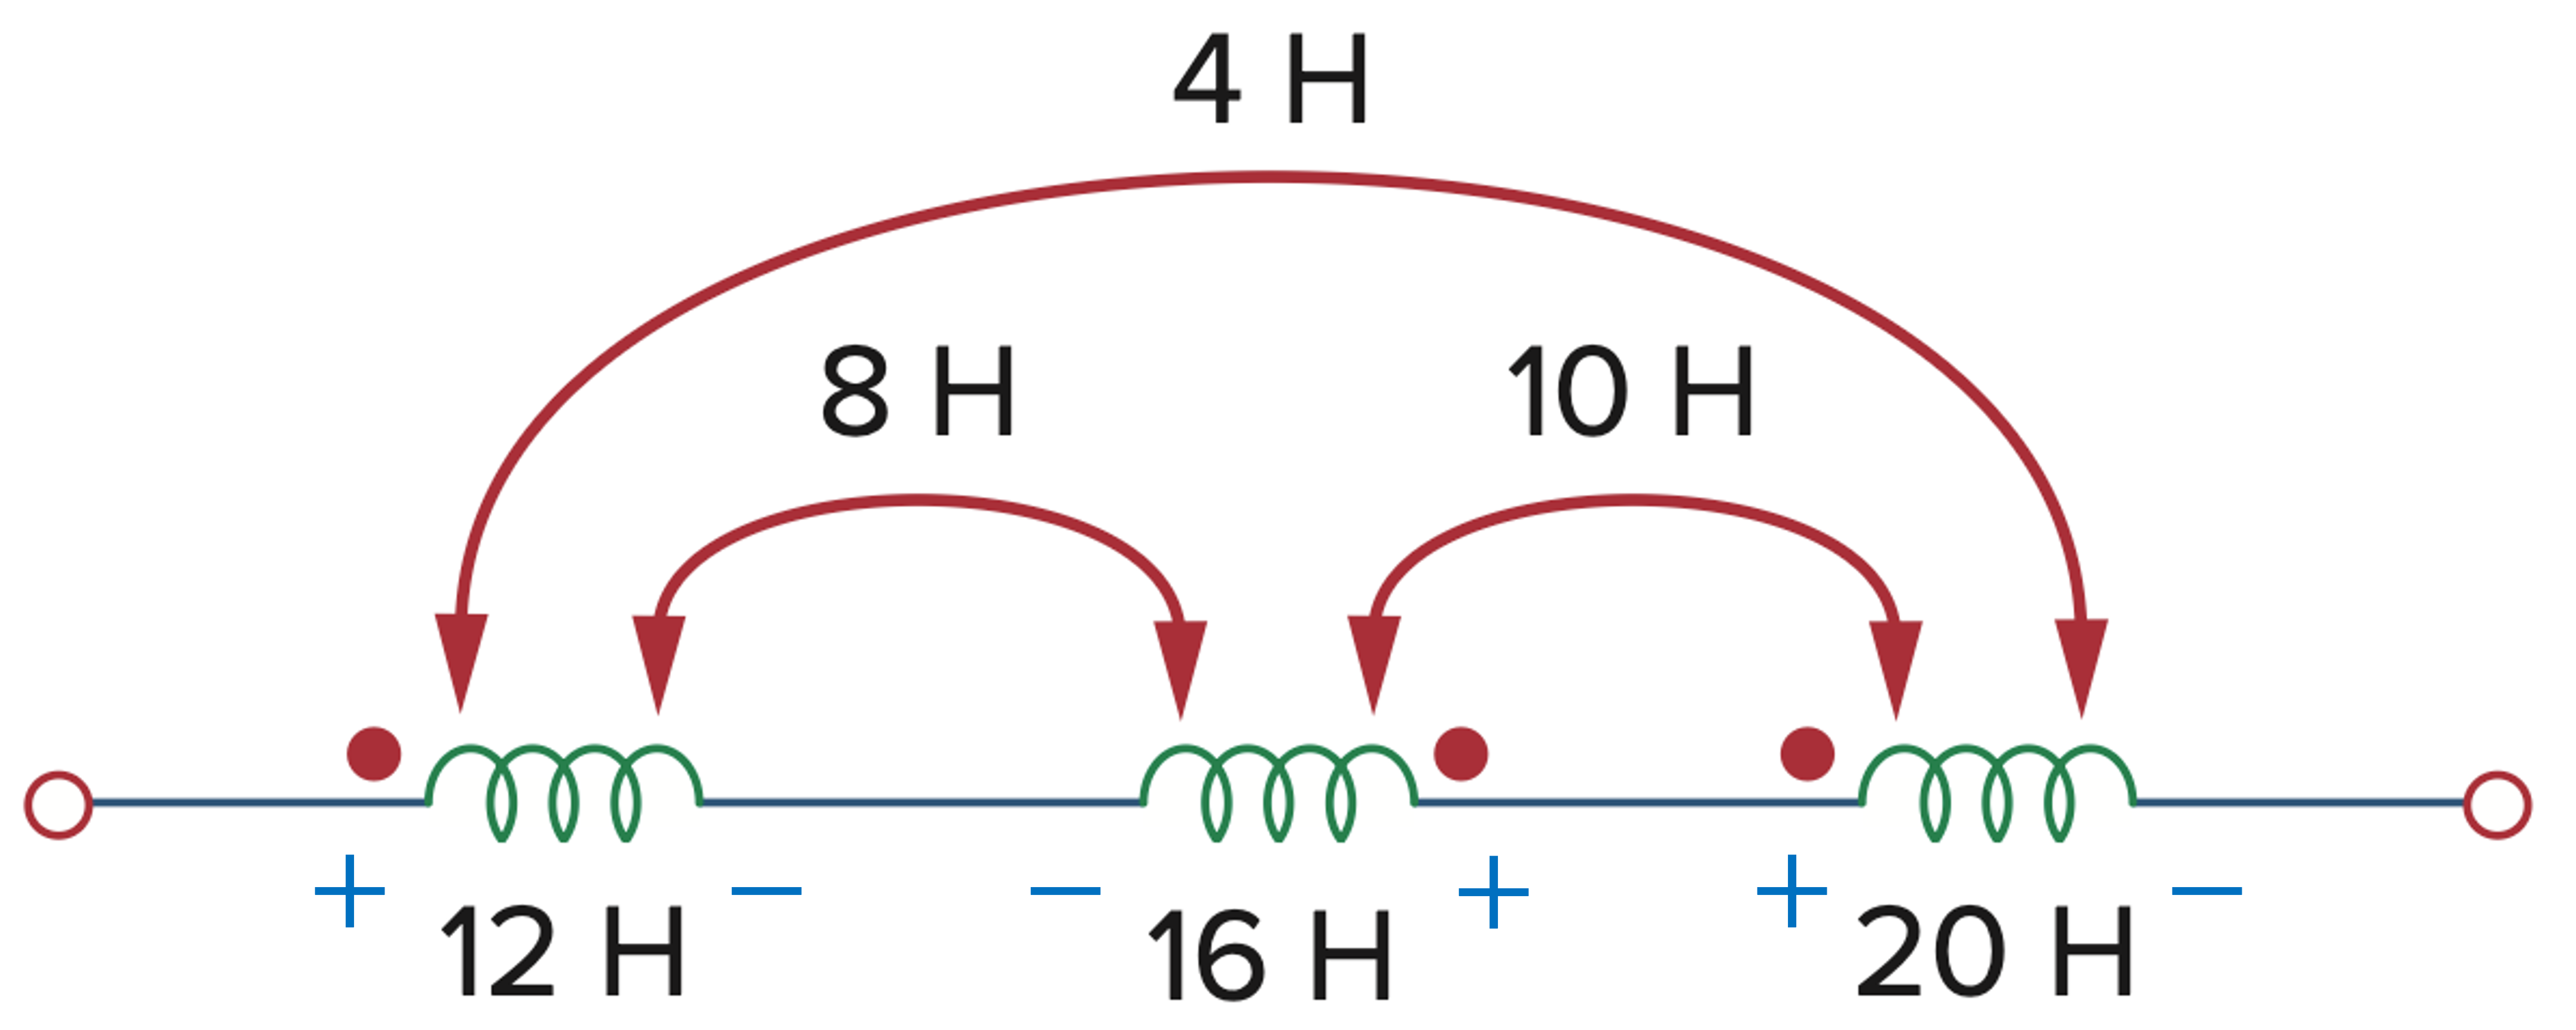
\includegraphics[width=0.7\textwidth]{figures/mutual_inductance_polarity.png}
\end{solution}
\fi

% ----- Exercise 8 -----
\begin{exercise}[RC-Discharge]
In the circuit shown below, for \(t>0\)
\[
v(t) = 56e^{-200t}\,\text{V},\qquad i(t) = 8e^{-200t}\,\text{mA}.
\]
\begin{enumerate}[label=\alph*)]
  \item Find the values of \(R\) and \(C\).
  \item Calculate the time constant \(\tau\).
  \item Determine the time required for the voltage to decay to half its initial value at \(t=0\).
\end{enumerate}

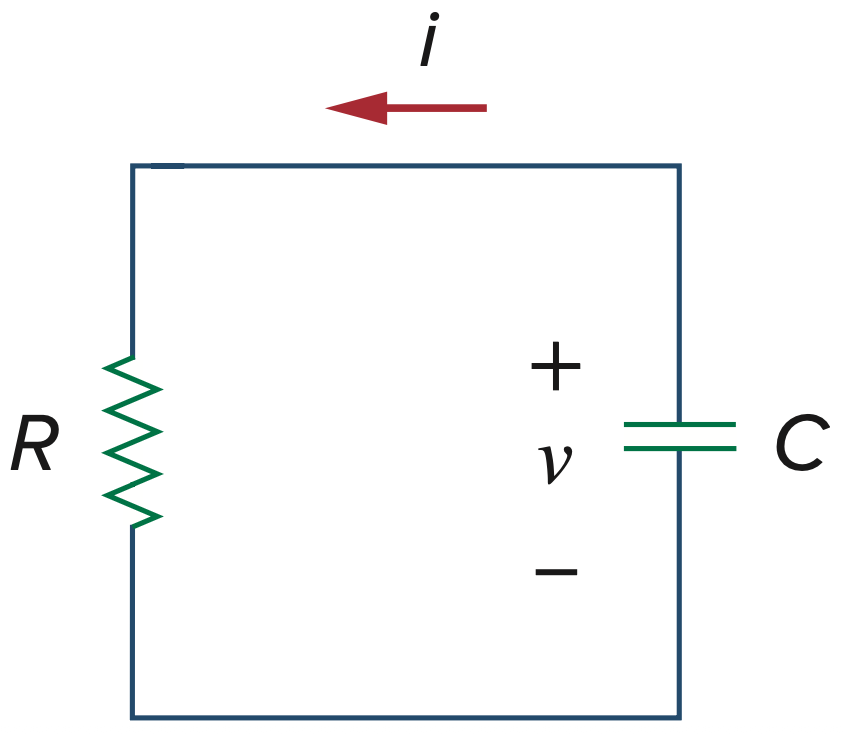
\includegraphics[width=0.5\textwidth]{figures/transients1.png}
\end{exercise}

\ifshowsolutions
\begin{solution}
\begin{enumerate}[label=\alph*)]
\item For a single series \(R\!-\!C\) discharge, the capacitor voltage has the form
\[
v(t) = V_0 e^{-t/(RC)}.
\]
Comparing \(v(t)=56e^{-200t}\) with \(V_0 e^{-t/(RC)}\) gives
\[
\frac{1}{RC} = 200 \quad\Longrightarrow\quad RC = 5\,\text{ms}.
\]

The capacitor current is related to the capacitor voltage by
\[
i(t) = C \frac{dv(t)}{dt}.
\]
Differentiate \(v(t)\):
\[
\frac{dv}{dt} = -200 \cdot 56 e^{-200t}\,\text{V/s} = -11200 e^{-200t}\,\text{V/s}.
\]
Hence
\[
C=\frac{i(t)}{dv/dt} = \frac{0.008 e^{-200t}}{-11200 e^{-200t}}.
\]
Taking the positive magnitude,
\[
C = \frac{0.008}{11200}\,\text{F} \approx 714.3\,\text{nF}.
\]

\[
R = \frac{RC}{C} = \frac{0.005}{714.3 \times 10^{-9}}\,\Omega = 7\,\text{k}\Omega
\]
(Alternatively, \(R = v(t)/i(t) = 56/0.008\,\Omega = 7\,\text{k}\Omega\).)

\item The time constant is
\[
\tau = RC = 5\,\text{ms}.
\]

\item We require \(v(t_{1/2}) = \tfrac{1}{2}V_0\). For \(v(t) = V_0 e^{-t/\tau}\),
\[
\frac{1}{2} = e^{-t_{1/2}/\tau}\quad\Longrightarrow\quad t_{1/2} = \tau \ln 2.
\]
Thus
\[
t_{1/2} = (0.005 \cdot \ln 2)\,\text{s} \approx 3.466\,\text{ms}.
\]
\end{enumerate}
\end{solution}
\fi

% ----- Exercise 9 -----
\begin{exercise}[Time Constant]
Determine the time constant for the circuit below.

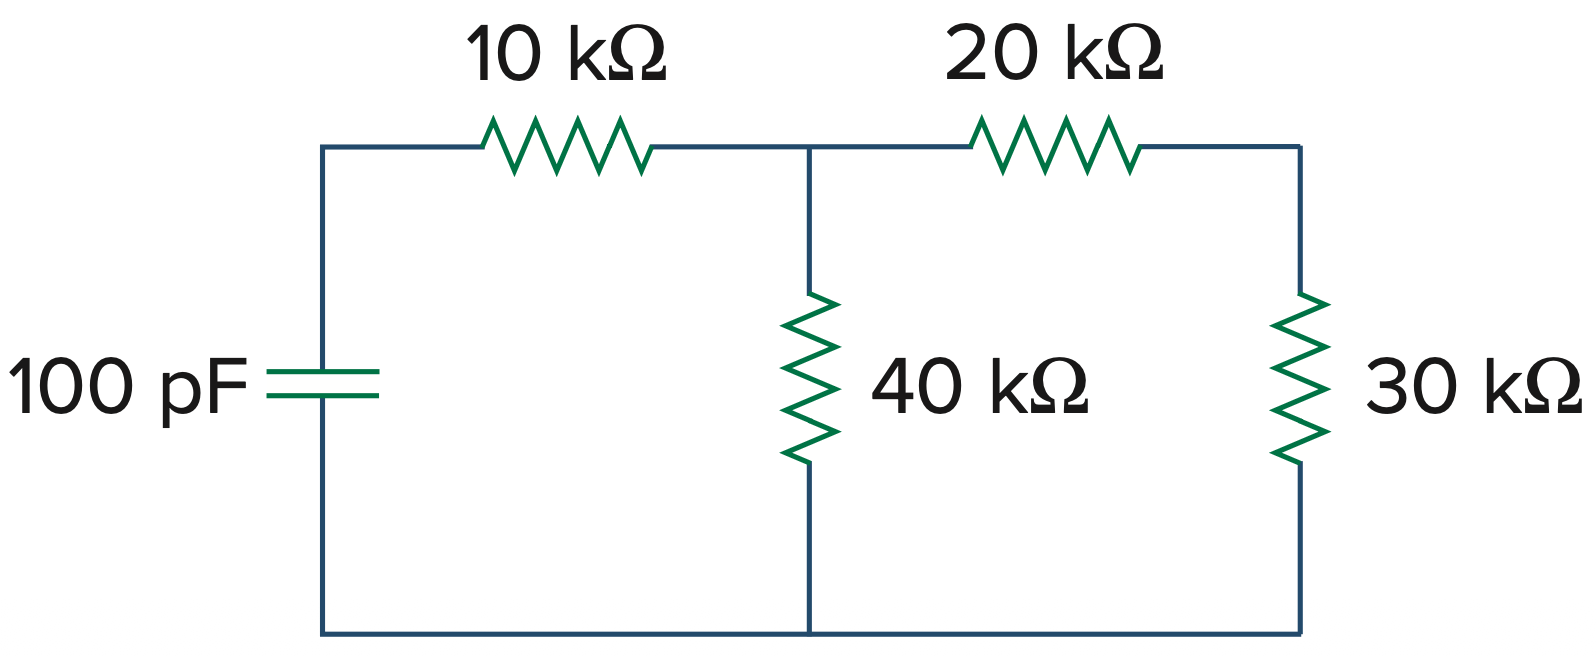
\includegraphics[width=0.7\textwidth]{figures/transients2.png}
\end{exercise}

\ifshowsolutions
\begin{solution}
Find the Thevenin resistance:
\[
R_{\text{th}} = 10~\text{k}\Omega + \left( 40~\text{k}\Omega \parallel (20~\text{k}\Omega + 30~\text{k}\Omega) \right) = 10~\text{k}\Omega + \frac{40 \cdot 50}{40 + 50}~\text{k}\Omega = \frac{290}{9}~\text{k}\Omega
\]

Compute the time constant:
\[
\tau = R_{\text{th}} C = \left( \frac{290}{9} \times 10^3~\Omega \right) \left( 100 \times 10^{-12}~\text{F} \right) = \frac{29000}{9} \times 10^{-9}~\text{s}
\]
\[
\tau \approx 3.22~\mu\text{s}
\]
\end{solution}
\fi

% ----- Exercise 10 -----
\begin{exercise}[Inductor Current Decay]
For the circuit below, find $i_o$ for $t > 0$.

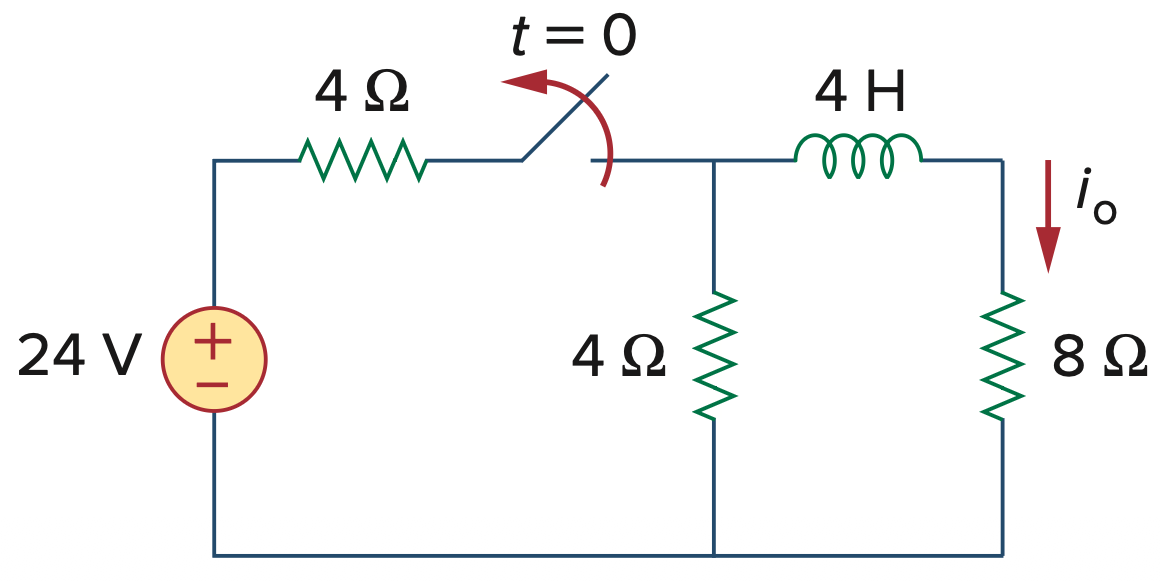
\includegraphics[width=0.7\textwidth]{figures/transients3.png}
\end{exercise}

\ifshowsolutions
\begin{solution}
The switch is closed for \(t<0\). Therefore, the inductor is in DC steady state and behaves as a short circuit.

The node after the left \(4\Omega\) resistor sees the parallel of \(4\Omega\) and \(8\Omega\):
\[
R_{\mathrm{eq}} = \frac{4 \cdot 8}{4+8} = \frac{8}{3}\ \Omega.
\]

The node voltage is
\[
v(0^-) = 24\,\frac{R_{\mathrm{eq}}}{4 + R_{\mathrm{eq}}} = 24\,\frac{8/3}{4 + 8/3} = 9.6\ \text{V}.
\]

Thus the inductor current at \(t=0^-\) is
\[
i_L(0^-) = \frac{v(0^-)}{8} = \frac{9.6}{8} = 1.2\ \text{A}.
\]

Therefore,
\[
i_L(0^+) = 1.2\ \text{A}.
\]

After the switch opens at \(t=0\), the source is disconnected. The top node is connected only to a \(4\Omega\) resistor to ground and the inductor with \(L=4\,\mathrm{H}\) in series with an \(8\Omega\) resistor.

Applying KCL at the top node (currents downward positive):
\[
\frac{v}{4} + i_L = 0
\]

Hence,
\[
v = -4 i_L.
\]

The right branch voltage is also
\[
v = 8 i_L + L \frac{di_L}{dt} = 8 i_L + 4\frac{di_L}{dt}.
\]

Equate the two expressions for \(v\):
\[
-4 i_L = 8 i_L + 4\frac{di_L}{dt}
\]

Divide by 4:
\[
\frac{di_L}{dt} + 3\, i_L = 0.
\]

Thus,
\[
i_L(t)= i_L(0^+)\, e^{-3t} = 1.2\, e^{-3t}.
\]

\[
\boxed{i_o(t)=1.2\,e^{-3t}\ \text{A},\quad t>0.}
\]
\end{solution}
\fi

% ----- Exercise 11 -----
\begin{exercise}[Energy Dissipation during Transient]
In the circuit below,
\[
v(t)=80e^{-10^{3}t}\ \text{V},\qquad t > 0,
\]
\[
i(t)=5e^{-10^{3}t}\ \text{mA},\qquad t > 0.
\]

\begin{enumerate}[label=\alph*)]
  \item Find \(R,\ L,\ \tau\).
  \item Calculate the energy dissipated in the resistance for \(0 < t < 0.5\,\text{ms}\).
\end{enumerate}

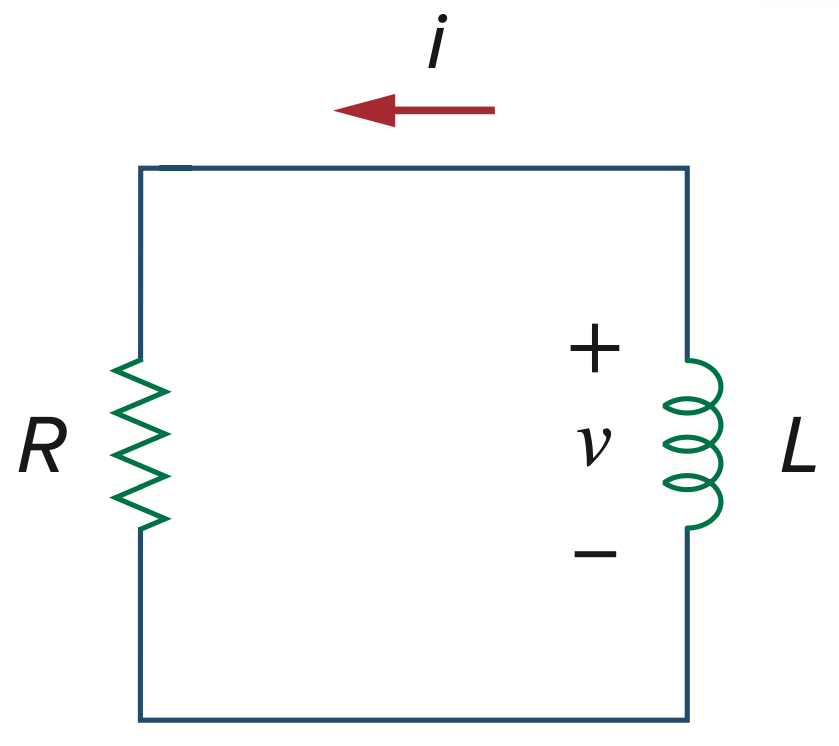
\includegraphics[width=0.7\textwidth]{figures/transients4.png}
\end{exercise}

\ifshowsolutions
\begin{solution}
\begin{enumerate}[label=\alph*)]
\item The current has the form \(i(t)=I_0 e^{-t/\tau}\). Comparing exponents,
\[
\frac{1}{\tau}=1000\quad\Longrightarrow\quad \tau = 1\,\text{ms}.
\]

Since \(v(t)\) is also the voltage across the resistor,
\[
R = \frac{v(t)}{i(t)} = \frac{80e^{-1000t}}{5\times10^{-3}e^{-1000t}} = 16\,\text{k}\Omega.
\]

Then
\[
L=\tau R=(1\times10^{-3})(1.6\times10^{4}) = 16\,\text{H}.
\]

\item The energy dissipated in \(R\) from \(t=0\) to \(t=t_1\) is
\[
W=\int_{0}^{t_1} i^2(t)\,R\,dt, \qquad t_1 = 0.5\,\text{ms}.
\]
Thus,
\[
W=R\int_0^{t_1} (5\times10^{-3})^2 e^{-2000t}\,dt = R\,(25\times10^{-6})\int_0^{t_1} e^{-2000t}\,dt.
\]
Evaluate the integral:
\[
\int_0^{t_1} e^{-2000t}\,dt=\left[-\frac{1}{2000}e^{-2000t}\right]_0^{t_1} =\frac{1}{2000}\big(1-e^{-2000t_1}\big).
\]
Therefore,
\[
W=R\,(25\times10^{-6})\frac{1}{2000}\big(1-e^{-2000t_1}\big).
\]
Substitute \(R=1.6\times10^{4}\) and \(2000t_1=2000(5\times10^{-4})=1\):
\[
W=(1.6\times10^{4})(25\times10^{-6})\frac{1}{2000}\big(1-e^{-1}\big) = 1.26424\times10^{-4}\,\text{J} \approx 0.126\ \text{mJ}.
\]
\end{enumerate}
\end{solution}
\fi

\end{document}